\PassOptionsToPackage{svgnames}{xcolor}
\documentclass[10pt,letterpaper]{article}
\usepackage[top=.5in, bottom=.75in, left=.5in, right=.5in]{geometry}
\usepackage{tcolorbox}
\usepackage{lipsum}
\tcbuselibrary{skins,breakable}
\usetikzlibrary{shadings,shadows}

\usepackage{graphicx} % Allows to include images
\usepackage{booktabs} % Allows the use of \toprule, \midrule and \bottomrule in tables

\usepackage{multicol}
\usepackage{float}

\usepackage[T1]{fontenc}
\usepackage[utf8]{inputenc}

\title{\vspace{-.5in}Practice 8: Killer Offense}
\author{\vspace{-.5in}}
\date{\vspace{-.5in}}

\newenvironment{agendablock}[1]{%
    \tcolorbox[beamer,%
    noparskip,breakable,
    colback=LightGray,colframe=Black,%
    colbacklower=Gray!75!LightGray,%
    title=#1]}%
    {\endtcolorbox}

\newenvironment{evenBlock}[1]{%
    \tcolorbox[beamer,%
    noparskip,breakable,
    colback=LightGreen,colframe=DarkGreen,%
    colbacklower=LimeGreen!75!LightGreen,%
    title=#1]}%
    {\endtcolorbox}

\newenvironment{oddBlock}[1]{%
    \tcolorbox[beamer,%
    noparskip,breakable,
    colback=LightBlue,colframe=DarkBlue,%
    colbacklower=DarkBlue!75!LightBlue,%
    title=#1]}%
    {\endtcolorbox}

\newenvironment{myexampleblock}[1]{%
    \tcolorbox[beamer,%
    noparskip,breakable,
    colback=LightGreen,colframe=DarkGreen,%
    colbacklower=LimeGreen!75!LightGreen,%
    title=#1]}%
    {\endtcolorbox}

\newenvironment{myalertblock}[1]{%
    \tcolorbox[beamer,%
    noparskip,breakable,
    colback=LightCoral,colframe=DarkRed,%
    colbacklower=Tomato!75!LightCoral,%
    title=#1]}%
    {\endtcolorbox}

\newenvironment{myblock}[1]{%
    \tcolorbox[beamer,%
    noparskip,breakable,
    colback=LightBlue,colframe=DarkBlue,%
    colbacklower=DarkBlue!75!LightBlue,%
    title=#1]}%
    {\endtcolorbox}

\usepackage{lmodern}

\begin{document}
\fontfamily{lmss}\selectfont


\maketitle

\begin{agendablock}{Practice Activities}
    \begin{enumerate}
        \item Warm ups / Coerver Touches [ 15 min ]
        \item Drills [ 35 min ]
        \item Small Sided Activity [ 15 min ]
        \item Small Sided Game [ 20 min ]
        \item Sprints [ 5 min ] 
    \end{enumerate}
\end{agendablock}

\section{Warm Ups}
Run the \textbf{CLOCKS} drill until everyone arrives and for a few minutes after.

\textbf{Time: 2 minutes}
\begin{evenBlock}{Clocks (10 min)}

\begin{minipage}[t]{\linewidth}
    \centering
    
    \begin{minipage}{.3\linewidth} % Left column and width
        \centering
        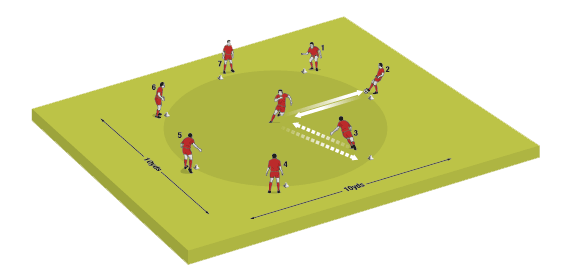
\includegraphics[width=\textwidth]{../img/Trimmed/Clocks1}
        \vspace{12pt}
        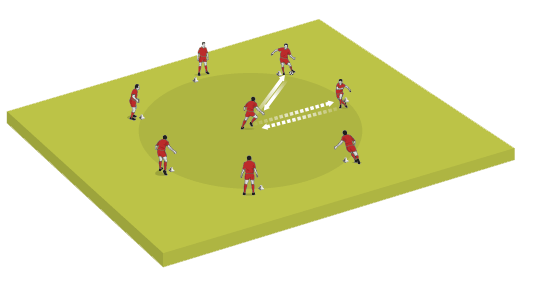
\includegraphics[width=\textwidth]{../img/Trimmed/Clocks2}
    \end{minipage}
    \hspace{0.05\linewidth}
    \begin{minipage}{.6\linewidth} % Left column and width
        \textbf{Drill Description:}
        Create a circle with your players of around 10 yards in diameter. Place cones around the circle where each player should stand, or go inside the centre circle and get the players to take a few steps forwards to get the right size. We’ve used eight players.
        \begin{enumerate}
        \setlength{\itemsep}{0pt}
        \setlength{\parskip}{0pt}
        \setlength{\parsep}{0pt}
        \item Start with the player in the middle who passes to one of the players around the circle
        \item Immediately the pass gets away, the centre player swaps position with the player clockwise from the player he passed to.
        \item The player he swaps with must get quickly into the centre to receive the ball and pass it to the next player anti-clockwise around the circle.
        \item Players continue to pass anti-clockwise and swap position with the player clockwise5. Try and get players to use one touch to get the ball around the clock
        \end{enumerate}
        
        \textbf{Coaching Points:}
        \begin{itemize}
        \setlength{\itemsep}{0pt}
        \setlength{\parskip}{0pt}
        \setlength{\parsep}{0pt}
        \item Focus on who gets your pass and then where you need to move.
        \item Attempt to complete this drill using a single touch.
        \end{itemize}

    \end{minipage}
\end{minipage}

\end{evenBlock}

%\textbf{Time: 3 minutes}
%\begin{myalertblock}{Theme of the Practice}
%    \textbf{Killer Offense!}
%
%    Importance of offense:
%    \begin{itemize}
%        \setlength{\itemsep}{0pt}
%        \setlength{\parskip}{0pt}
%        \setlength{\parsep}{0pt}
%        \item Good Offense prevents us from losing the game.
%        \item Offense allows good advancements in tournaments.
%    \end{itemize}
%
%    Some keys to good offense:
%    \begin{itemize}
%        \setlength{\itemsep}{0pt}
%        \setlength{\parskip}{0pt}
%        \setlength{\parsep}{0pt}
%        \item Ball possession,
%        \item good ball movement,
%        \item perfect player movement when the player is not on the ball.
%        \item player movement with the ball.
%    \end{itemize}
%
%    Ball possession is important because:
%    \begin{itemize}
%        \setlength{\itemsep}{0pt}
%        \setlength{\parskip}{0pt}
%        \setlength{\parsep}{0pt}
%        \item it allows us to control the location of the ball on the pitch,
%        \item allows us setup a score.
%    \end{itemize}
%
%    Good ball movement is important because:
%    \begin{itemize}
%        \setlength{\itemsep}{0pt}
%        \setlength{\parskip}{0pt}
%        \setlength{\parsep}{0pt}
%        \item it forces the other team to move.  A passed ball can travel faster than any player on the field, so good ball movement can move the other team off the ball and open up a scoring opportunity.
%        \item sets up excellent scoring opportunities.
%    \end{itemize}
%
%    Player movement off the ball is important because:
%    \begin{itemize}
%        \setlength{\itemsep}{0pt}
%        \setlength{\parskip}{0pt}
%        \setlength{\parsep}{0pt}
%        \item with out good player movement off the ball make ball movement is difficult.
%        \item Correct player movement off the ball can setup more open shots on goal than dribbling.
%    \end{itemize}
%
%    Player movement with the ball is important because:
%    \begin{itemize}
%        \setlength{\itemsep}{0pt}
%        \setlength{\parskip}{0pt}
%        \setlength{\parsep}{0pt}
%        \item it can be used to pull the defense to the ball setting up ball movement to open space.
%        \item good dribbling moves can create space to allow for a good pass or shot.
%    \end{itemize}
%
%\end{myalertblock}

\textbf{Time: 10 minutes}
\begin{agendablock}{Captain Led Warm ups / Coerver Touches (15 min) }
    \textbf{Warmups}
    \begin{enumerate}
        \item Jog to the 18 yard line and back twice with your ball (inside cut first time, outside cut the second),
        \item Side-Step to 18 yd line and back twice,
        \item Butt Kickers to the 18 yd line and back twice,
        \item Jog Backwards to the 18 yd line and back twice.
    \end{enumerate}
    \textbf{Touches}
    \begin{enumerate}
        \item Toe-Touches (20 count alternating feet).
        \item Pull back and Push Forward (10 each foot).
        \item Side to Side or Pendulums (20 count).
        \item Triangles (10 each foot).
        \item Pullback-Behind (20 count).
    \end{enumerate}
\end{agendablock}

\section{HOWTO:}
\begin{evenBlock}{HOWTO:  Shoot Hard (5 min)}

\begin{minipage}[t]{\linewidth}
    \centering
    Review these elements prior to beginning the passing drills so its fresh in their heads.

    %\begin{minipage}{.3\linewidth} % Left column and width
        %\centering
        %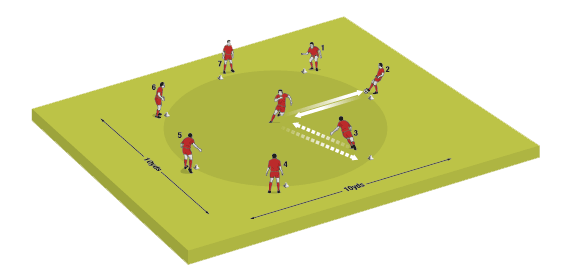
\includegraphics[width=\textwidth]{../img/Trimmed/Clocks1}
    %\end{minipage}
    %\hspace{0.05\linewidth}
    %\begin{minipage}{.6\linewidth} % Left column and width
    
        \textbf{Elements of the Power Kicking:}
    
        \begin{enumerate}
        \setlength{\itemsep}{0pt}
        \setlength{\parskip}{0pt}
        \setlength{\parsep}{0pt}
        \item Ball should be in front of the player.
        \item Non-kicking leg should be planted next to the ball with passer's toe pointed at the target.
        \item Ball should be struck with a locked ankle, the toe is pointed downward, exposing the top of the foot.  The top of the fot is the hardest part of the foot and when it strikes the ball - will impart the most energy into the ball.
        \item The kick should have a large follow through - ideally the kicker lands on his kicking foot.
        \item Landing on your kicking foot imparts all of the kickers body weight into the ball.
        \end{enumerate}
        
        \textbf{Elements of the Power Kicking:}
    
        \begin{enumerate}
        \setlength{\itemsep}{0pt}
        \setlength{\parskip}{0pt}
        \setlength{\parsep}{0pt}
        \item Ball should be in front of the player.
        \item Non-kicking leg should be planted next to the ball with passer's toe pointed at the target.
        \item Ball should be struck with a locked ankle, the toe is pointed downward, exposing the top of the foot.  The top of the fot is the hardest part of the foot and when it strikes the ball - will impart the most energy into the ball.
        \item The kick should have a large follow through - ideally the kicker lands on his kicking foot.
        \item Landing on your kicking foot imparts all of the kickers body weight into the ball.
        \end{enumerate}
    %\end{minipage}
\end{minipage}

\end{evenBlock}

\section{Drills}

\textbf{Time: 10 minutes}
\begin{evenBlock}{Get the Snitch}

\begin{minipage}[t]{\linewidth}
    \centering
    
    \begin{minipage}{.5\linewidth} % Left column and width
        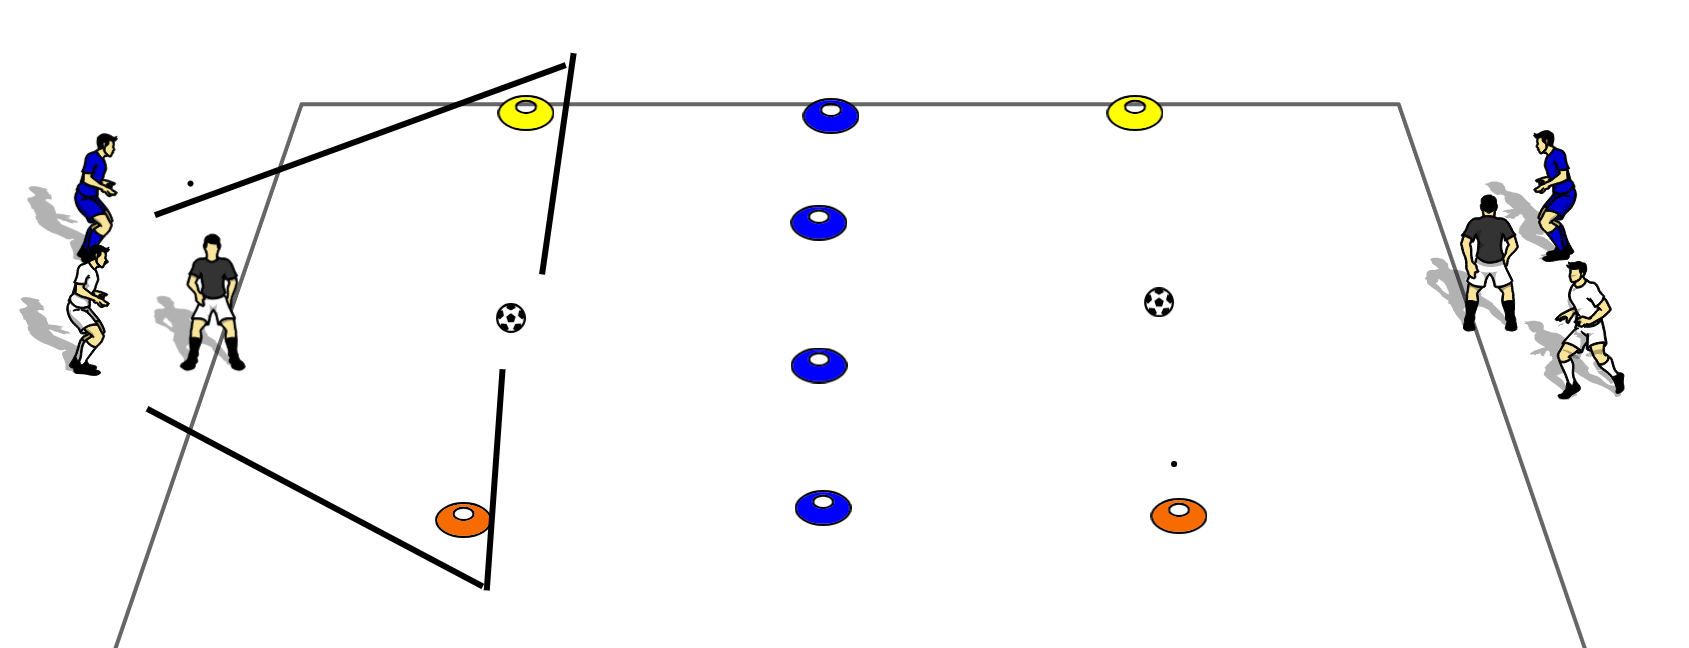
\includegraphics[width=\textwidth]{../img/Trimmed/Get_the_Snitch}
    \end{minipage}
    \hspace{0.05\linewidth}
    \begin{minipage}{.4\linewidth} % Left column and width
        \textbf{Drill Description:}
        The object is to get the ball (the snitch) and take it across the opposite end line.
        \begin{enumerate}
            \setlength{\itemsep}{0pt}
            \setlength{\parskip}{0pt}
            \setlength{\parsep}{0pt}
            \item Coach calls go and kicks a ball into the field, both players race around their cone to get to the ball.
            \item First player to get the ball tries to drive across the fair end line while the other player defends that line.
        \end{enumerate}
    \end{minipage}
\end{minipage}
\vspace{12pt}

%\textbf{Coaching Points:}
%\begin{itemize}
%    \setlength{\itemsep}{0pt}
%    \setlength{\parskip}{0pt}
%    \setlength{\parsep}{0pt}
%    \item Explain marking a player is to remain within 2 or 3 feet of the attacking player.
%    \item Explain how to mark a player goal side (defender between the attacker and goal).
%    \item Attackers try to lose their marks by passing.
%\end{itemize}
\end{evenBlock}

\textbf{Time: 10 minutes}
\begin{evenBlock}{1v1 Evade with Help}

\begin{minipage}[t]{\linewidth}
    \centering
    
    \begin{minipage}{.5\linewidth} % Left column and width
        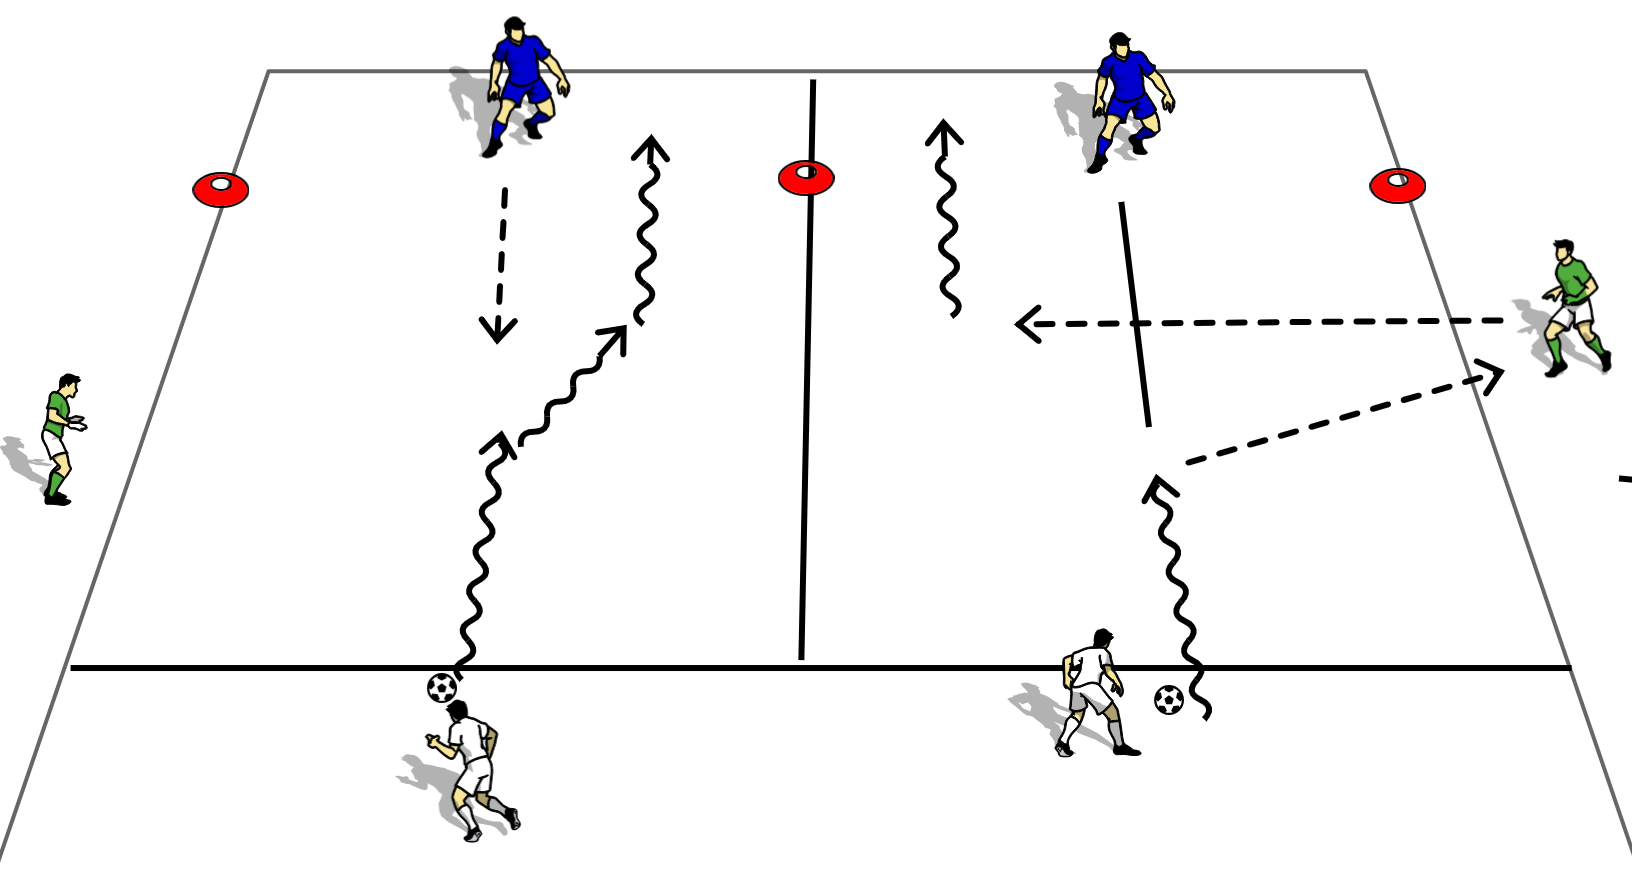
\includegraphics[width=\textwidth]{../img/Trimmed/Evade_1V1+Help}
    \end{minipage}
    \hspace{0.05\linewidth}
    \begin{minipage}{.4\linewidth} % Left column and width
        \textbf{Drill Description:}
        The object is to get the ball (the snitch) and take it across the opposite end line.
        \begin{enumerate}
            \setlength{\itemsep}{0pt}
            \setlength{\parskip}{0pt}
            \setlength{\parsep}{0pt}
            \item Player with the ball crosses the far end line and ties to dribble across the opposite endline.
            \item A defender starts behind the red cones and can cross them as soon as the attacker enters the box.
            \item The attacker needs to evade the defender or pass to his helper (coach) on the side line, who one touches the ball back into play.
        \end{enumerate}
    \end{minipage}
\end{minipage}
\vspace{12pt}

\textbf{Coaching Points:}
\begin{itemize}
    \setlength{\itemsep}{0pt}
    \setlength{\parskip}{0pt}
    \setlength{\parsep}{0pt}
    \item The timing of the attacking move is critical, it needs to be early enough to insure the defender can't block it, but not so early the defender can react to counter it.
    \item Use the pass as a great opportunity to evade the defender.
\end{itemize}
\end{evenBlock}

\textbf{Time: 15 minutes}
\begin{evenBlock}{2 vs. 1 Offense (10 min)}


\begin{minipage}[t]{\linewidth}
    \centering
    
    \begin{minipage}{.3\linewidth} % Left column and width
        %\begin{figure}
            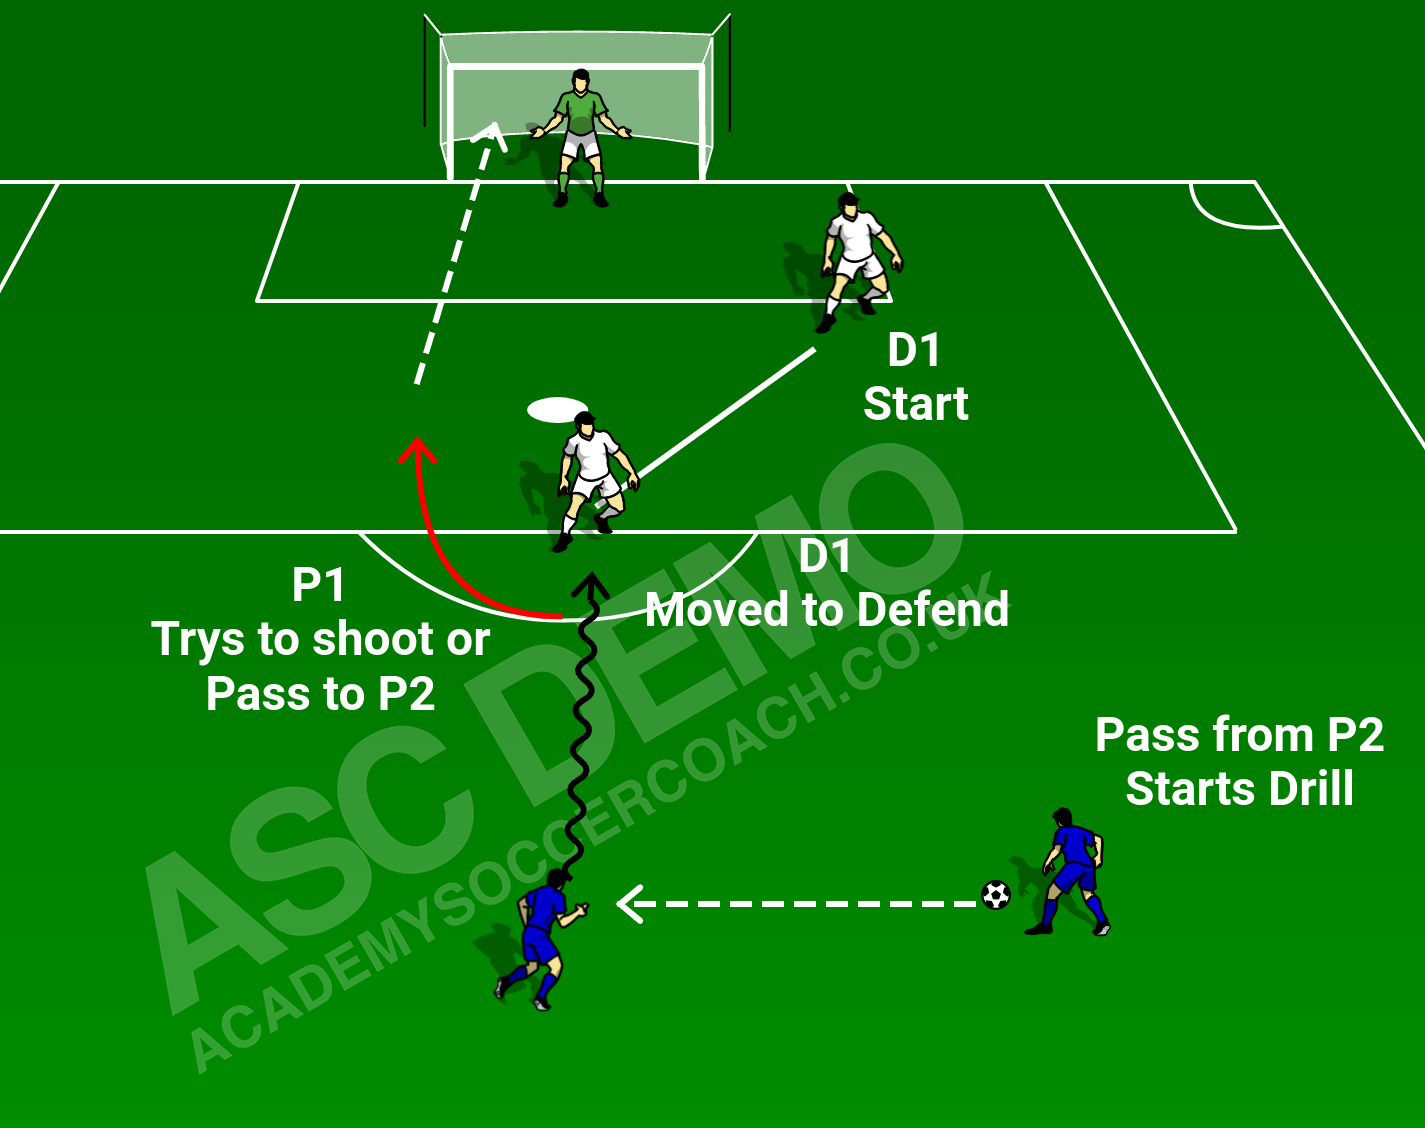
\includegraphics[width=\textwidth]{../img/Trimmed/2v1_Option}

            \vspace{3pt}
            
            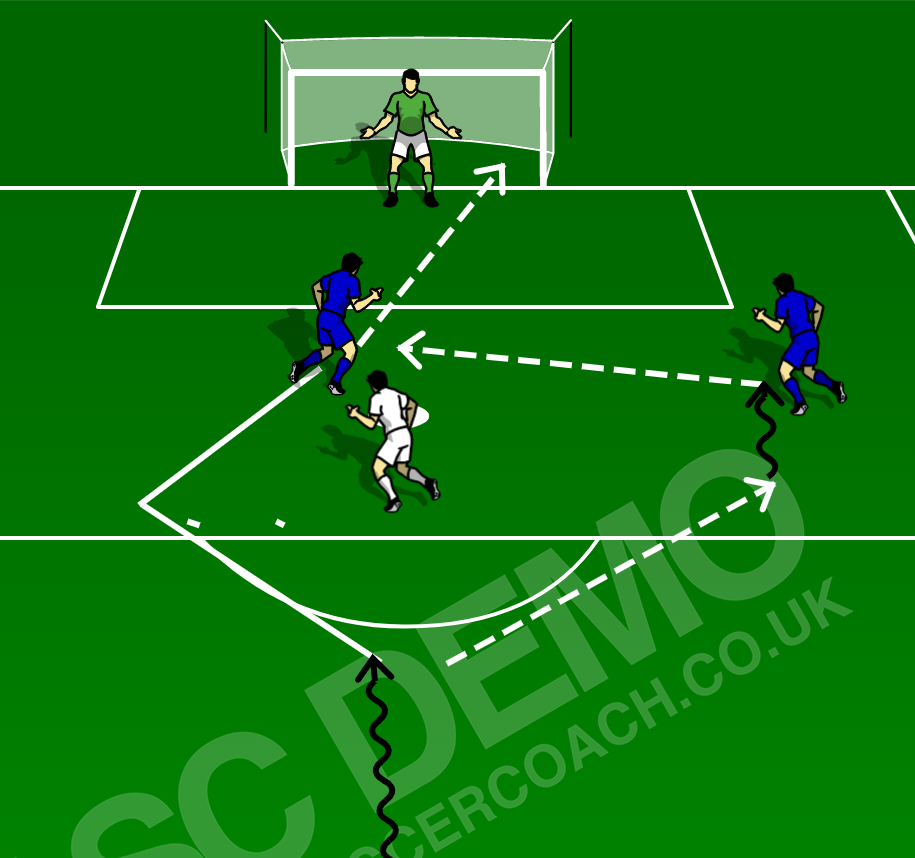
\includegraphics[width=\textwidth]{../img/Trimmed/2v1_Option_Pass}
        %    \caption{Drill: 4 Person Passing}
        %\end{figure}
    \end{minipage}
    \hspace{0.05\linewidth}
    \begin{minipage}{.6\linewidth} % Left column and width
        \textbf{Drill Description:}
        This drill is designed train the forward to make a quick decision on how to beat a defender.  He has two options, dribble around the defender or pass to his wing and make a move around the defender. 
        \begin{enumerate}
        \setlength{\itemsep}{0pt}
        \setlength{\parskip}{0pt}
        \setlength{\parsep}{0pt}
        \item The wing (P2) starts the play by passing to the forward.  The defender (D1) starts at the corner of the 6 yard box.
        \item The forward drives to goal as a defender come charging to defend.
        \item The forward has two choices, pass or make a move/touch around the defender.
        \item The goal is to get a shot on goal.
        \item If he passes the ball, the wing should cross the ball quickly as the striker is passing the defender.
        \end{enumerate}

        \vspace{3pt}
        
        Rotate rolls each shot: P2 to P1, P1 to D1, D1 to P2.

        \vspace{10pt}
        
        \textbf{Coaching Points:}
        \begin{itemize}
        \setlength{\itemsep}{0pt}
        \setlength{\parskip}{0pt}
        \setlength{\parsep}{0pt}
        \item The forward needs to decide quickly which option he plans to take.
        \item The wing needs to be ready at all times and should stay `on-side'.
        \item The forward should try and take advantage of any weakness of the defense, or try and create weakness by using a scissor move or a fake.
        \item Explain on-sides and off-sides.
        \end{itemize}

    \end{minipage}
\end{minipage}

\end{evenBlock}

\section{Small Sided Activity}
\textbf{Time: 15 minutes, Started at 1:15 PM to 1:20 PM}
\begin{evenBlock}{3v2+Keeper}

\begin{minipage}[t]{\linewidth}
    \centering
    
    \begin{minipage}{.5\linewidth} % Left column and width
        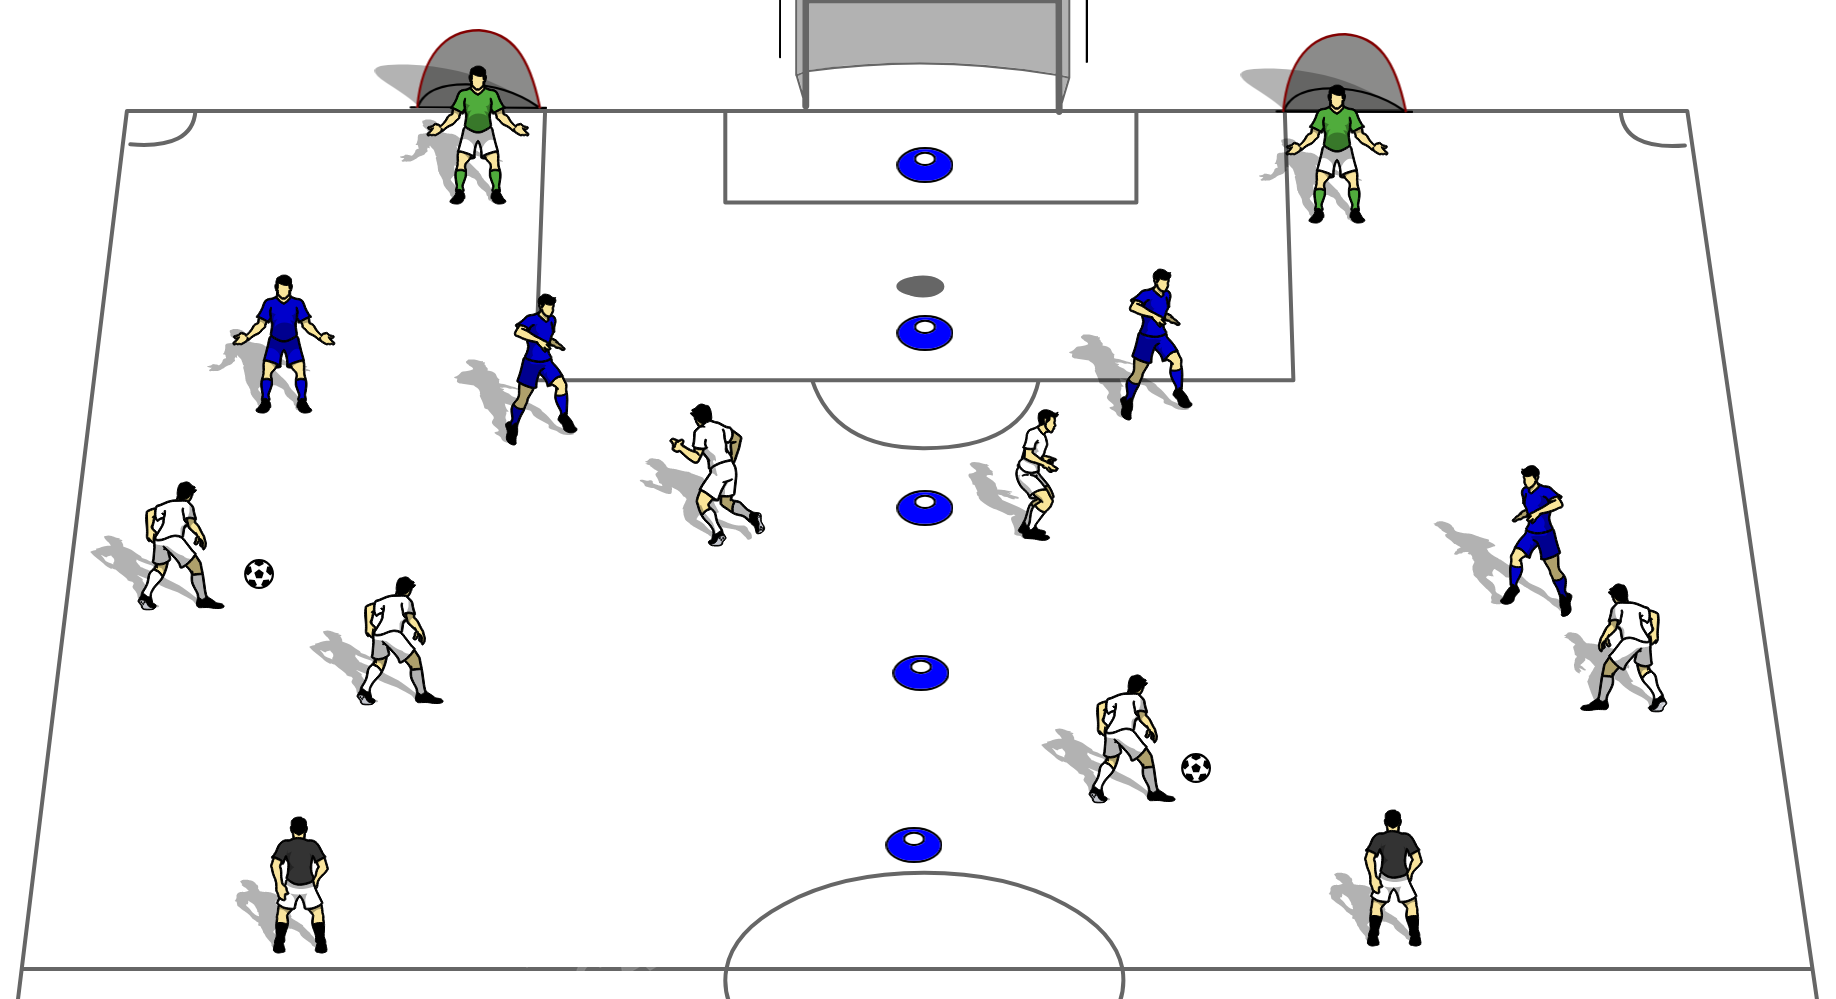
\includegraphics[width=\textwidth]{../img/Trimmed/3v2+Keeper}
    \end{minipage}
    \hspace{0.05\linewidth}
    \begin{minipage}{.4\linewidth} % Left column and width
        \textbf{Drill Description:}
        This drill requires 6 players + 1 coach or 12 players and 2 coaches.
        \begin{enumerate}
            \setlength{\itemsep}{0pt}
            \setlength{\parskip}{0pt}
            \setlength{\parsep}{0pt}
            \item The defending team uses 2 defenders and 1 keeper.
            \item Attacking team has 3 and tries to score on the small defended goal.
            \item The defending team scores by completing a pass to the coach on the center line.
        \end{enumerate}
    \end{minipage}
\end{minipage}
\vspace{12pt}

\textbf{Coaching Points:}
\begin{itemize}
    \setlength{\itemsep}{0pt}
    \setlength{\parskip}{0pt}
    \setlength{\parsep}{0pt}
    \item Explain marking a player is to remain within 2 or 3 feet of the attacking player.
    \item Explain how to mark a player goal side (defender between the attacker and goal).
    \item Attackers try to lose their marks by passing.
\end{itemize}
\end{evenBlock}

\section{Game}

\textbf{Start Time: 1:35 PM}

\begin{oddBlock}{Small Sided}
    \textbf{Time:} 10 minute halves.

    \textbf{Size:} 4v4 or 5v5.

    Express:
    \begin{itemize}
        \setlength{\itemsep}{0pt}
        \setlength{\parskip}{0pt}
        \setlength{\parsep}{0pt}
        \item  remind them about the practice goals and expectation there is a lot of movement and passing.
        \item Funnel Positioning.
        \item Go outside on our defensive half.
        \item Pass quickly down sidelines or into open space.
        \item Avoid passing backward.
        \item Make a pass early or move early.
    \end{itemize}

\end{oddBlock}

\section{Close}
\begin{oddBlock}{Sprints (5 min)}
    Agility runs to cone 5 yards away, stop and step circling cone then explode to next cone, circling it then explode sprinting to half field, jog back to end line and repeat 3 times.
\end{oddBlock}

\end{document}